
\item During an experiment with a metre bridge, the galvanometer shows a null point when the jockey is pressed at 40.0 cm using a standard resistance of 90 \(\Omega\), as shown in the figure. The least count of the scale used in the metre bridge is 1 mm. The unknown resistance is
    \begin{center}
        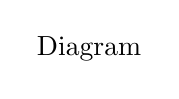
\begin{tikzpicture}
            \node at (0, 0) {Diagram}; % Replace this with the actual TikZ code for the diagram
        \end{tikzpicture}
    \end{center}
    \begin{tasks}(2)
        \task \(60 \pm 0.15\Omega\)
        \task \(135 \pm 0.56\Omega\)
        \task \(60 \pm 0.25\Omega\)
        \task \(135 \pm 0.23\Omega\)
    \end{tasks}
